\chapter{Metodología}

\section{Diseño de la Investigación}
\subsection{Tipo y alcance de la investigación}
La presente investigación se enmarca en un alcance exploratorio-correlacional-explicativo. Como señala \cite{hernandez2020metodologia}, este enfoque multicapa permite:

\begin{itemize}
    \item \textbf{Fase exploratoria:} Identificar variables y patrones iniciales en los datos históricos de comportamiento crediticio, examinando factores que podrían influir en la morosidad.
    \item \textbf{Fase correlacional:} Establecer relaciones estadísticas entre las variables identificadas y el comportamiento de pago, cuantificando su influencia relativa.
    \item \textbf{Fase explicativa:} Desarrollar modelos predictivos que expliquen y anticipen el riesgo de morosidad, proporcionando una base para intervenciones preventivas.
\end{itemize}

Este enfoque resulta particularmente adecuado para abordar la complejidad del comportamiento crediticio en el sector mayorista, donde intervienen múltiples variables interrelacionadas.

\subsection{Enfoque metodológico}
La investigación adopta un enfoque predominantemente cuantitativo, basado en el análisis de datos históricos de comportamiento de pago y variables asociadas. Este enfoque se complementa con elementos cualitativos para la interpretación contextual de los resultados, considerando factores del sector mayorista ecuatoriano que podrían no estar completamente capturados en los datos numéricos.

\section{Aplicación de la Metodología CRISP-DM}
\subsection{Fase 1: Comprensión del negocio}
\subsubsection{Contexto organizacional}
La empresa objeto de estudio opera en el sector mayorista de productos de juguetería, hogar, aseo y cocina en Ecuador. Con una trayectoria de más de 15 años en el mercado, gestiona una cartera crediticia que supera el millón de dólares, distribuida entre 238 clientes activos a nivel nacional.

\subsubsection{Objetivos de negocio}
Los objetivos de negocio que motivan esta investigación incluyen:

\begin{itemize}
    \item Reducir la tasa de morosidad en al menos un 20\% respecto a los niveles actuales
    \item Optimizar la asignación de cupos de crédito basada en análisis predictivo del comportamiento
    \item Implementar un sistema de alertas tempranas que permita intervenciones preventivas
    \item Automatizar el proceso de evaluación de riesgo para nuevos clientes y ampliaciones de cupo
\end{itemize}

\subsubsection{Evaluación de la situación actual}
Actualmente, la empresa utiliza métodos tradicionales para la evaluación crediticia, basados principalmente en:

\begin{itemize}
    \item Historial de pagos
    \item Referencias comerciales
    \item Tiempo como cliente
    \item Volumen promedio de compras
\end{itemize}

Este enfoque presenta limitaciones significativas:

\begin{itemize}
    \item Baja capacidad predictiva (precisión estimada del 60\%)
    \item Evaluación reactiva más que preventiva
    \item Escasa consideración de factores externos (estacionalidad, geografía)
    \item Proceso manual con alta dependencia del criterio individual
\end{itemize}

\subsubsection{Determinación de objetivos de minería de datos}
Con base en la comprensión del negocio, se establecen los siguientes objetivos específicos para el proceso de minería de datos:

\begin{itemize}
    \item Identificar los factores con mayor poder predictivo para anticipar riesgo de morosidad
    \item Desarrollar un modelo predictivo con precisión superior al 80\%
    \item Segmentar la cartera de clientes según perfiles de riesgo
    \item Generar indicadores tempranos de alerta para cada segmento
\end{itemize}

\subsection{Fase 2: Comprensión de los datos}
\subsubsection{Descripción de las fuentes de datos}
Los datos para esta investigación provienen de múltiples fuentes internas de la empresa:

\begin{itemize}
    \item \textbf{Sistema ERP:} Datos transaccionales de ventas, devoluciones y pagos desde 2017
    \item \textbf{CRM:} Información de clientes, incluyendo datos demográficos y geográficos
    \item \textbf{Sistema de cobranzas:} Registros históricos de gestión de cobro y comportamiento de pago
    \item \textbf{Hojas de cálculo complementarias:} Registros manuales de seguimiento de cartera
\end{itemize}

\subsubsection{Exploración inicial de datos}
La exploración inicial revela un conjunto de datos con las siguientes características:

\begin{itemize}
    \item \textbf{Volumen:} Aproximadamente 150,000 registros transaccionales
    \item \textbf{Período:} Datos históricos desde enero 2017 hasta diciembre 2024
    \item \textbf{Granularidad:} Nivel transaccional (facturas, pagos, notas de crédito)
    \item \textbf{Dimensiones geográficas:} Distribución en 12 provincias del Ecuador
    \item \textbf{Categorías de productos:} 4 líneas principales (juguetería, hogar, aseo, cocina)
\end{itemize}

\subsubsection{Verificación de calidad de datos}
La evaluación preliminar de calidad de datos identifica los siguientes aspectos:

\begin{table}[ht]
\centering
\begin{tabular}{|p{4cm}|p{3cm}|p{7cm}|}
\hline
\textbf{Aspecto} & \textbf{Estado} & \textbf{Observaciones} \\
\hline
Completitud & Parcial & Datos faltantes en aproximadamente 12\% de los registros, principalmente en campos descriptivos y categorización de productos \\
\hline
Consistencia & Moderada & Inconsistencias en la codificación de regiones geográficas y en la clasificación de motivos de retraso \\
\hline
Precisión & Alta en datos financieros & Los montos y fechas de transacciones muestran alta precisión, mientras que los datos cualitativos presentan mayor variabilidad \\
\hline
Actualización & Diaria para transacciones & Los sistemas transaccionales se actualizan diariamente, mientras que la información complementaria tiene actualizaciones variables \\
\hline
\end{tabular}
\caption{Evaluación de calidad de datos}
\end{table}

\subsection{Fase 3: Preparación de los datos}
\subsubsection{Selección de datos}
Con base en la exploración inicial y los objetivos establecidos, se seleccionan las siguientes variables para el análisis:

\begin{table}[ht]
\centering
\begin{tabular}{|p{4cm}|p{3cm}|p{7cm}|}
\hline
\textbf{Variable} & \textbf{Tipo} & \textbf{Descripción} \\
\hline
ID\_Cliente & Categórica & Identificador único de cliente \\
\hline
Región & Categórica & Ubicación geográfica (provincia) \\
\hline
Antigüedad & Numérica & Tiempo como cliente (meses) \\
\hline
Promedio\_Compra & Numérica & Monto promedio de compra mensual \\
\hline
Frecuencia\_Compra & Numérica & Número promedio de compras por mes \\
\hline
Días\_Promedio\_Pago & Numérica & Tiempo promedio para completar pagos \\
\hline
Máximo\_Días\_Atraso & Numérica & Máximo retraso histórico en días \\
\hline
Porcentaje\_Devoluciones & Numérica & Porcentaje de mercadería devuelta \\
\hline
Categoría\_Principal & Categórica & Línea de producto predominante \\
\hline
Índice\_Estacionalidad & Numérica & Variación estacional en compras \\
\hline
Historial\_Mora & Categórica & Clasificación histórica de comportamiento \\
\hline
\end{tabular}
\caption{Variables seleccionadas para el análisis}
\end{table}

\subsubsection{Limpieza de datos}
El proceso de limpieza incluye las siguientes acciones:

\begin{itemize}
    \item \textbf{Tratamiento de valores faltantes:} Imputación mediante técnicas estadísticas para variables numéricas y moda para variables categóricas
    \item \textbf{Identificación y manejo de valores atípicos:} Aplicación del método IQR (Rango Intercuartílico) para detectar outliers y su normalización
    \item \textbf{Estandarización de codificaciones:} Unificación de categorías geográficas y de productos
    \item \textbf{Validación de coherencia temporal:} Corrección de inconsistencias en secuencias temporales de transacciones
\end{itemize}

\subsubsection{Construcción y transformación de variables}
A partir de los datos disponibles, se derivan las siguientes variables adicionales:

\begin{itemize}
    \item \textbf{Ratio\_Pago\_Plazo:} Relación entre días reales de pago y plazo acordado
    \item \textbf{Variabilidad\_Pago:} Desviación estándar en comportamiento de pago
    \item \textbf{Índice\_Concentración\_Producto:} Diversificación de compras entre categorías
    \item \textbf{Tendencia\_Compra:} Pendiente de evolución de montos de compra (últimos 6 meses)
    \item \textbf{Índice\_Cumplimiento:} Ratio ponderado de cumplimiento de compromisos de pago
\end{itemize}

Las transformaciones aplicadas include:

\begin{itemize}
    \item Normalización Min-Max para variables numéricas
    \item Codificación One-Hot para variables categóricas
    \item Transformación logarítmica para variables con distribución sesgada
    \item Discretización de variables continuas para análisis específicos
\end{itemize}

\subsubsection{Integración de datos}
La integración de las diversas fuentes se realiza mediante un proceso ETL (Extracción, Transformación, Carga) que combina:

\begin{itemize}
    \item Exportación programada de datos transaccionales
    \item Carga incremental de nuevos registros
    \item Consolidación en una estructura unificada de datos
    \item Verificación de integridad referencial entre fuentes
\end{itemize}

El resultado es un conjunto de datos integrado con 238 registros (uno por cliente) y 32 variables (originales y derivadas).
\subsubsection{Arquitectura del Data Warehouse implementado}

Para materializar el proceso ETL y soportar el análisis predictivo de morosidad, se diseñó e implementó un Data Warehouse corporativo utilizando SQL Server 2022 como motor de base de datos. La arquitectura adoptada sigue el paradigma de modelo dimensional tipo estrella (star schema), reconocido por su eficiencia en consultas analíticas y su claridad conceptual para usuarios de negocio \cite{kimball2013toolkit}.

\textbf{Organización por esquemas}

El Data Warehouse se estructura en cinco esquemas lógicos que separan responsabilidades y facilitan el mantenimiento del sistema:

\begin{enumerate}
    \item \textbf{Esquema STAGING:} Zona de aterrizaje para datos de origen. Contiene ocho sinónimos que proporcionan acceso de solo lectura a las vistas transaccionales de la base de datos operacional (siinf\_casalindap\_ec), incluyendo información de clientes, facturas, pagos y devoluciones. Esta capa de abstracción permite realizar las transformaciones ETL sin impactar el rendimiento del sistema de producción.
    
    \item \textbf{Esquema DIM:} Almacena las siete dimensiones del modelo. Implementa la técnica Slowly Changing Dimensions Tipo 2 (SCD-2) para cinco de las dimensiones (Cliente, Producto, Punto de Venta, Campaña y Tipo de Pago), permitiendo mantener un historial completo de cambios en los atributos descriptivos \cite{kimball2008scd}. Las dimensiones restantes (Tiempo y Estado) son de tipo estático.
    
    \item \textbf{Esquema FACT:} Contiene las tres tablas de hechos principales: FactFacturas (con aproximadamente 85,242 registros de transacciones de venta), FactPagos (con 14,356 registros de recaudación) y FactDevoluciones (estructura preparada para datos futuros). Cada tabla de hechos almacena métricas cuantitativas y claves foráneas hacia las dimensiones correspondientes.
    
    \item \textbf{Esquema ETL:} Proporciona la infraestructura de control y auditoría del sistema. Incluye cinco tablas: LogEjecucion (bitácora de procesos), CalidadDatos (métricas de validación), ControlCargaIncremental (gestión de cargas incrementales), ConfiguracionProcesos (parámetros de ejecución) y ErroresDetallados (registro de excepciones). Este esquema garantiza la trazabilidad completa de todas las operaciones ETL.
    
    \item \textbf{Esquema ML:} Dedicado al soporte de machine learning, contiene las tablas DatasetMorosidad (568 registros con 35 features calculados), Predicciones (resultados del modelo) y ModelosRegistro (versionado de algoritmos y métricas de rendimiento).
\end{enumerate}

\textbf{Modelo dimensional}

El modelo dimensional implementado responde a la pregunta de negocio central: ¿cómo analizar el comportamiento de morosidad de clientes considerando múltiples perspectivas? La estructura resultante permite analizar las métricas de morosidad desde siete ángulos diferentes:

\begin{table}[ht]
\centering
\begin{tabular}{|p{3cm}|p{4cm}|p{7.5cm}|}
\hline
\textbf{Dimensión} & \textbf{Registros} & \textbf{Análisis que facilita} \\
\hline
DimTiempo & 5,844 & Tendencias temporales, estacionalidad, análisis por períodos \\
\hline
DimCliente & 1,407 & Segmentación por tipo, ubicación geográfica, vendedor asignado \\
\hline
DimProducto & 4,127 & Comportamiento por línea de producto, categoría \\
\hline
DimPuntoVenta & 2 & Comparación entre canales de distribución \\
\hline
DimCampana & 83 & Impacto de campañas comerciales en morosidad \\
\hline
DimTipoPago & 8 & Relación entre forma de pago y comportamiento crediticio \\
\hline
DimEstado & 23 & Estados del ciclo de vida de documentos \\
\hline
\end{tabular}
\caption{Dimensiones del modelo y su propósito analítico}
\end{table}

Las tablas de hechos almacenan las métricas cuantitativas esenciales para el análisis de morosidad. En FactFacturas se registran los montos facturados, saldos pendientes, días de mora y clasificación del estado crediticio. FactPagos complementa esta información con datos de recaudación, puntualidad de pago y retenciones aplicadas. Esta estructura permite realizar análisis tanto retrospectivos como prospectivos del comportamiento crediticio.

\textbf{Implementación de Slowly Changing Dimensions Tipo 2}

Para capturar la evolución histórica de los atributos de las entidades de negocio, se implementó SCD Tipo 2 en cinco dimensiones clave. Esta técnica agrega tres campos de control a cada tabla: FechaInicioVigencia (timestamp de inicio de validez del registro), FechaFinVigencia (timestamp de fin de validez, NULL para registro activo) y EsRegistroActual (flag booleano que identifica la versión vigente).

Cuando se detecta un cambio en algún atributo descriptivo de una dimensión, el sistema automáticamente marca el registro anterior como histórico (estableciendo FechaFinVigencia y EsRegistroActual = 0) e inserta un nuevo registro con los valores actualizados. Este mecanismo preserva la integridad histórica permitiendo analizar el comportamiento de morosidad considerando las características que el cliente tenía en cada momento del tiempo.

\subsubsection{Proceso ETL automatizado}

El proceso de Extracción, Transformación y Carga (ETL) se implementó mediante procedimientos almacenados en SQL Server que ejecutan automáticamente todas las fases del pipeline de datos. El diseño modular permite ejecutar procesos individuales o la cadena completa, facilitando tanto las cargas iniciales como las actualizaciones incrementales.

\textbf{Arquitectura de procedimientos almacenados}

Se desarrollaron doce procedimientos almacenados organizados en tres niveles jerárquicos:

\begin{enumerate}
    \item \textbf{Procedimientos de dimensión individual:} Siete procedimientos especializados, uno por cada dimensión del modelo. Cada procedimiento implementa la lógica específica de transformación y, cuando corresponde, el algoritmo SCD Tipo 2.
    
    \item \textbf{Procedimientos de hechos:} Tres procedimientos que cargan las tablas de hechos, realizando las validaciones de integridad referencial necesarias y calculando las métricas derivadas.
    
    \item \textbf{Procedimientos maestros:} Dos procedimientos de orquestación (sp\_CargarTodasDimensiones y sp\_CargarTodosHechos) que ejecutan las cargas en el orden correcto considerando las dependencias entre tablas.
\end{enumerate}

\textbf{Fases del proceso ETL}

El proceso completo de ETL se ejecuta en cinco fases secuenciales:

\paragraph{Fase 1: Extracción}
La extracción de datos se realiza mediante consultas sobre los sinónimos del esquema STAGING, que apuntan a las vistas materializadas del sistema transaccional. Este enfoque de sinónimos proporciona dos ventajas clave: primero, desacopla el Data Warehouse del sistema fuente, permitiendo modificaciones en las rutas o nombres sin alterar el código ETL; segundo, minimiza el impacto en el rendimiento del sistema operacional al evitar consultas directas sobre las tablas transaccionales.

\paragraph{Fase 2: Transformación de dimensiones}
Las dimensiones se cargan en orden considerando las dependencias conceptuales. El proceso inicia con DimTiempo, que genera automáticamente el calendario completo desde el año 2020 hasta 2030, incluyendo los días festivos oficiales de Ecuador. Posteriormente se cargan DimCliente, DimProducto, DimPuntoVenta, DimCampana, DimTipoPago y DimEstado.

Para las dimensiones con SCD Tipo 2, el proceso ejecuta tres operaciones:
\begin{itemize}
    \item Identifica registros nuevos (que no existen en la dimensión)
    \item Detecta cambios en registros existentes mediante comparación de checksums
    \item Procesa historización, marcando el registro antiguo como no vigente e insertando el nuevo registro con vigencia actual
\end{itemize}

\paragraph{Fase 3: Transformación de hechos}
La carga de tablas de hechos implementa lógica de negocio específica para el análisis de morosidad. Para FactFacturas, se calculan automáticamente tres campos derivados críticos: Dias\_Mora (diferencia entre fecha actual y fecha de vencimiento), Es\_Moroso (indicador binario que marca facturas con saldo pendiente y mora mayor a cero días) y Rango\_Mora (clasificación en categorías: "Al Día", "1-30 días", "31-60 días", "61-90 días", "91-120 días", ">120 días"). Estos campos derivados eliminan la necesidad de cálculos repetitivos en las consultas analíticas.

Para FactPagos, el proceso implementa lógica de consolidación que resuelve el problema de múltiples formas de pago por transacción. Cuando un pago utiliza combinaciones de efectivo, cheque, transferencia u otros instrumentos, el sistema selecciona la forma de pago principal mediante una regla de priorización basada en el monto más alto.

\paragraph{Fase 4: Preparación de dataset de machine learning}
El procedimiento ml.sp\_PrepararDataset realiza agregaciones a nivel de cliente calculando 35 features que sintetizan el comportamiento histórico crediticio. Este proceso transforma los datos transaccionales granulares en un dataset analítico optimizado para algoritmos de clasificación.

Los features se organizan en cinco categorías: comportamiento histórico (diez variables sobre patrones de pago), métricas financieras (ocho variables de montos y ratios), tendencias temporales (ocho variables de actividad reciente), contexto categórico (seis variables de segmentación) y variable objetivo (tres variantes del indicador de morosidad). El procedimiento también realiza la división aleatoria de los registros en conjuntos de entrenamiento (70\%), validación (15\%) y prueba (15\%) para facilitar el proceso de modelado.

\paragraph{Fase 5: Control de calidad y auditoría}
Cada ejecución de procedimiento ETL genera automáticamente registros de auditoría en las tablas del esquema ETL. La tabla LogEjecucion almacena metadatos de cada ejecución: nombre del proceso, timestamps de inicio y fin, duración, cantidad de registros procesados/insertados/actualizados y estado final (Completado/Error). En caso de excepciones, los detalles completos del error se registran en ErroresDetallados incluyendo el mensaje de error, stack trace y datos de contexto.

\textbf{Optimizaciones implementadas}

El proceso ETL incorpora varias optimizaciones que mejoran significativamente el rendimiento:

\begin{itemize}
    \item \textbf{Índices estratégicos:} Creación de índices no agrupados en columnas frecuentemente utilizadas en JOINs y cláusulas WHERE
    \item \textbf{Carga incremental:} La tabla ControlCargaIncremental rastrea la última fecha procesada para cada fuente, permitiendo cargar únicamente los registros nuevos o modificados
    \item \textbf{Particionamiento de consultas:} Las cargas masivas se dividen en lotes de 10,000 registros para evitar bloqueos prolongados
    \item \textbf{Transaccionalidad:} Uso de transacciones explícitas con manejo de rollback para garantizar consistencia
\end{itemize}

La implementación completa del proceso ETL toma aproximadamente 60-90 minutos para la carga inicial de datos históricos (2017-2024), mientras que las actualizaciones incrementales diarias se completan en 15-25 minutos.

\subsection{Fase 4: Modelado}
\subsubsection{Selección de técnicas de modelado}
Con base en los objetivos del proyecto y la naturaleza de los datos, se seleccionan las siguientes técnicas de modelado:

\begin{table}[ht]
\centering
\begin{tabular}{|p{3.5cm}|p{3.5cm}|p{7cm}|}
\hline
\textbf{Técnica} & \textbf{Propósito} & \textbf{Justificación} \\
\hline
Regresión Logística & Modelo base de clasificación & Ofrece interpretabilidad y establece una línea base de rendimiento \\
\hline
Random Forest & Clasificación avanzada & Alta precisión y capacidad para manejar variables correlacionadas \\
\hline
XGBoost & Clasificación optimizada & Rendimiento superior en problemas de clasificación binaria \\
\hline
K-Means & Segmentación de clientes & Identificación de grupos naturales en la cartera según perfil de riesgo \\
\hline
Redes Neuronales & Exploración de relaciones complejas & Capacidad para capturar interacciones no lineales entre variables \\
\hline
\end{tabular}
\caption{Técnicas de modelado seleccionadas}
\end{table}

\subsubsection{Diseño de pruebas}
El enfoque de validación incluye:

\begin{itemize}
    \item \textbf{División de datos:} 70\% entrenamiento, 30\% prueba
    \item \textbf{Validación cruzada:} K-fold (k=5) para estimación robusta del rendimiento
    \item \textbf{Técnicas de remuestreo:} SMOTE para abordar el desbalance de clases
    \item \textbf{Evaluación secuencial:} Entrenamiento progresivo con datos cronológicos para simular implementación real
\end{itemize}

\subsubsection{Construcción de modelos}
Para cada técnica seleccionada, se implementan los siguientes pasos:

\begin{enumerate}
    \item Inicialización con configuración base
    \item Entrenamiento inicial con conjunto de entrenamiento
    \item Ajuste de hiperparámetros mediante Grid Search o Bayesian Optimization
    \item Reentrenamiento con configuración optimizada
    \item Evaluación con métricas múltiples
\end{enumerate}

\subsubsection{Evaluación y comparación de modelos}
La evaluación de los modelos se realiza utilizando las siguientes métricas:

\begin{itemize}
    \item Exactitud (Accuracy)
    \item Precisión (Precision)
    \item Sensibilidad (Recall)
    \item F1-Score
    \item Área bajo la curva ROC (AUC)
    \item Pérdida logarítmica (Log Loss)
    \item Tiempo de entrenamiento y predicción
\end{itemize}

Adicionalmente, se evalúa la relevancia de las variables (feature importance) para cada modelo, lo que proporciona insights sobre los factores más determinantes en la predicción de morosidad.
% ============================================================================
% SECCIÓN ADICIONAL PARA METODOLOGÍA.TEX
% Agregar después de la sección de CRISP-DM - Fase 4: Modelado
% ============================================================================

\subsection{Implementación Técnica del Modelo XGBoost}

La implementación práctica del modelo predictivo se realizó mediante un conjunto integrado de scripts Python que conectan directamente con el Data Warehouse construido en SQL Server, garantizando una arquitectura robusta y escalable para la predicción automatizada de morosidad.

\subsubsection{Arquitectura de la Solución}

La arquitectura implementada sigue un patrón de capas claramente definidas que separa las responsabilidades y facilita el mantenimiento del sistema. En la capa de persistencia, SQL Server 2022 aloja tanto el Data Warehouse operacional como el esquema especializado de machine learning, que incluye las tablas DatasetMorosidad para el conjunto de datos de entrenamiento, Predicciones para almacenar los resultados del modelo, y ModelosRegistro para mantener un histórico de versiones y métricas de cada modelo entrenado.

La capa de procesamiento analítico, implementada en Python 3.8, utiliza bibliotecas especializadas para cada aspecto del pipeline de machine learning. La biblioteca pandas gestiona la manipulación eficiente de datos tabulares, mientras que numpy proporciona operaciones matriciales de alto rendimiento. Para la conectividad con SQL Server, se emplea pyodbc con el driver ODBC 17, garantizando compatibilidad y rendimiento óptimo en las operaciones de lectura y escritura masiva de datos.

El componente de machine learning propiamente dicho se construye sobre scikit-learn para la preparación de datos, validación cruzada y evaluación de modelos, mientras que la biblioteca xgboost proporciona la implementación optimizada del algoritmo de gradient boosting. Las bibliotecas matplotlib y seaborn se utilizan para la generación de visualizaciones analíticas de los resultados del modelo.

\subsubsection{Proceso de Entrenamiento del Modelo}

El script principal de entrenamiento implementa un pipeline completo que abarca desde la extracción de datos hasta la persistencia del modelo entrenado. El proceso inicia con la conexión a SQL Server mediante autenticación Windows, estableciendo una sesión robusta que maneja automáticamente la reconexión en caso de interrupciones temporales.

La extracción del dataset se realiza mediante una consulta SQL optimizada que recupera todos los registros de la tabla DatasetMorosidad, la cual contiene aproximadamente quinientos sesenta y ocho observaciones con treinta y dos variables predictoras. Estas variables incluyen métricas de comportamiento crediticio como días promedio de atraso histórico, desviación estándar de los días de atraso, y ratio de facturas vencidas, complementadas con variables contextuales como región geográfica codificada, mes de análisis para capturar estacionalidad, y antigüedad del cliente en días.

Una vez cargado el dataset en memoria como un DataFrame de pandas, se procede con la división estratificada en tres conjuntos independientes. El conjunto de entrenamiento comprende el sesenta por ciento de los datos y se utiliza para el ajuste inicial de los parámetros del modelo. El conjunto de validación, con veinte por ciento de las observaciones, sirve para la optimización de hiperparámetros mediante validación cruzada. Finalmente, el conjunto de prueba, con el veinte por ciento restante de los datos, se reserva exclusivamente para la evaluación final del modelo, garantizando una estimación imparcial del rendimiento en datos completamente no vistos durante el entrenamiento.

La normalización de características numéricas se implementa mediante StandardScaler de scikit-learn, que transforma cada variable a media cero y desviación estándar uno. Esta normalización es crucial para algoritmos basados en gradientes como XGBoost, ya que asegura que todas las variables contribuyan equitativamente al modelo independientemente de sus escalas originales. El objeto scaler se persiste junto con el modelo para garantizar que los datos de predicción futura reciban exactamente la misma transformación.

\subsubsection{Optimización de Hiperparámetros}

La optimización de hiperparámetros se realiza mediante GridSearchCV, que implementa una búsqueda exhaustiva en el espacio de parámetros definido. La grilla de búsqueda incluye combinaciones de learning rate entre cero punto cero uno y cero punto tres, profundidad máxima de árboles entre tres y siete niveles, número de estimadores entre cincuenta y doscientos, y el parámetro de subsample entre cero punto ocho y uno punto cero.

Para cada combinación de hiperparámetros, se realiza validación cruzada estratificada con cinco pliegues, garantizando que la distribución de la clase positiva (clientes morosos) se mantenga equilibrada en cada pliegue. El criterio de optimización seleccionado es el F1-score, que proporciona un balance apropiado entre precisión y recall, particularmente importante en problemas de clasificación desbalanceada como la predicción de morosidad donde los casos positivos son minoritarios.

El proceso de búsqueda exhaustiva evalúa aproximadamente cuarenta y ocho combinaciones de parámetros, requiriendo entre una y tres horas de tiempo computacional dependiendo de las características del hardware disponible. Durante la ejecución, el sistema muestra mensajes informativos sobre el progreso de la búsqueda y las mejores configuraciones encontradas hasta el momento.

\subsubsection{Evaluación y Métricas del Modelo}

Una vez identificada la configuración óptima de hiperparámetros, se reentrena el modelo sobre el conjunto completo de entrenamiento más validación, y se evalúa su rendimiento sobre el conjunto de prueba reservado. Las métricas de evaluación incluyen accuracy para medir la proporción general de predicciones correctas, precision para cuantificar la confiabilidad de las predicciones positivas (clientes identificados como morosos que efectivamente lo son), recall para medir la capacidad del modelo de identificar todos los casos positivos reales, F1-score como media armónica entre precision y recall, y área bajo la curva ROC (AUC-ROC) como medida integral de discriminación entre clases.

La matriz de confusión generada proporciona un desglose detallado de verdaderos positivos, falsos positivos, verdaderos negativos y falsos negativos, permitiendo analizar los tipos específicos de errores que comete el modelo. Esta información es crucial para determinar si el modelo tiende a ser conservador (clasificando pocos casos como morosos, minimizando falsos positivos) o agresivo (clasificando muchos casos como morosos, minimizando falsos negativos).

El análisis de importancia de variables se realiza mediante el método de ganancia acumulada de información, que cuantifica la contribución de cada variable al poder predictivo del modelo. Este análisis revela que las variables de comportamiento histórico de pago (días promedio de atraso, desviación estándar de atraso, ratio de facturas vencidas) tienen la mayor importancia predictiva, seguidas por variables contextuales como región geográfica y estacionalidad.

\subsubsection{Persistencia y Versionado del Modelo}

El modelo entrenado se persiste mediante la biblioteca joblib, que utiliza un protocolo de serialización optimizado para objetos Python complejos. El archivo resultante contiene no solo el modelo XGBoost entrenado, sino también el objeto StandardScaler con los parámetros de normalización, los encoders para variables categóricas, y metadatos completos incluyendo las métricas de rendimiento, los hiperparámetros seleccionados, la fecha y hora de entrenamiento, y la versión de las bibliotecas utilizadas.

Simultáneamente, se registra una entrada en la tabla ModelosRegistro de SQL Server, creando un histórico auditable de todas las versiones del modelo entrenadas. Este registro incluye un identificador único del modelo, timestamp de creación, métricas de rendimiento en formato JSON, y la ruta al archivo del modelo persistido. Esta práctica de versionado es esencial en entornos productivos, permitiendo rastrear la evolución del rendimiento del modelo a lo largo del tiempo y facilitar rollbacks si una nueva versión presenta degradación en el rendimiento.

\subsubsection{Generación de Predicciones}

El script de predicción implementa un pipeline complementario que carga el modelo persistido más reciente y genera predicciones para el conjunto actual de clientes activos. El proceso inicia cargando el modelo desde disco, verificando la integridad del archivo y la compatibilidad de versiones de las bibliotecas.

Los datos para predicción se extraen de una vista SQL que integra información del Data Warehouse, calculando en tiempo real las mismas características utilizadas durante el entrenamiento. Es crítico que las definiciones de estas características sean idénticas a las del entrenamiento para evitar discrepancias que degradarían el rendimiento predictivo (fenómeno conocido como training-serving skew).

Cada predicción incluye no solo la clasificación binaria (moroso o no moroso), sino también la probabilidad estimada de morosidad, lo que permite establecer umbrales de decisión flexibles según el apetito de riesgo de la organización. Los resultados se clasifican en niveles de riesgo (bajo, medio, alto, muy alto) basados en percentiles de probabilidad, y se asignan acciones recomendadas específicas para cada nivel (desde monitoreo estándar hasta intervención inmediata de cobranza).

Las predicciones se escriben directamente a la tabla Predicciones en SQL Server, incluyendo timestamp de generación, identificador del modelo utilizado, probabilidad de morosidad, nivel de riesgo clasificado, y acción recomendada. Esta tabla se convierte en la fuente de datos principal para el dashboard de Power BI, cerrando el ciclo desde los datos transaccionales hasta la visualización de alertas tempranas accionables.

\subsection{Fase 5: Evaluación}
\subsubsection{Evaluación de resultados respecto a objetivos de negocio}
Los resultados obtenidos se evalúan en relación con los objetivos de negocio establecidos:

\begin{itemize}
    \item \textbf{Reducción de morosidad:} Estimación de impacto potencial basada en la capacidad predictiva
    \item \textbf{Optimización de asignación de cupo:} Evaluación de recomendaciones generadas por el modelo
    \item \textbf{Efectividad de alertas tempranas:} Tiempo de anticipación logrado por las predicciones
    \item \textbf{Automatización del proceso:} Viabilidad técnica y operativa de la implementación
\end{itemize}

\subsubsection{Revisión del proceso}
Se realiza una revisión integral del proceso seguido, identificando:

\begin{itemize}
    \item Lecciones aprendidas en cada fase
    \item Desafíos metodológicos enfrentados
    \item Adaptaciones realizadas a la metodología estándar
    \item Áreas de mejora para futuras iteraciones
\end{itemize}

\subsection{Fase 6: Implementación}
\subsubsection{Plan de implementación}
La implementación del modelo seleccionado contempla las siguientes etapas:

\begin{enumerate}
    \item \textbf{Desarrollo de API:} Creación de interfaces programáticas para integración con sistemas existentes
    \item \textbf{Diseño de dashboard:} Desarrollo de interfaz de visualización para usuarios finales
    \item \textbf{Automatización de actualización:} Implementación de procesos de reentrenamiento periódico
    \item \textbf{Documentación técnica:} Elaboración de manuales y guías de referencia
    \item \textbf{Capacitación:} Formación a usuarios en interpretación y uso de resultados
\end{enumerate}

\subsubsection{Monitoreo y mantenimiento}
El plan de monitoreo y mantenimiento incluye:

\begin{itemize}
    \item Seguimiento continuo del rendimiento del modelo
    \item Alertas automáticas ante degradación de precisión
    \item Actualización trimestral con nuevos datos de comportamiento
    \item Revisión semestral de variables y parámetros
    \item Procedimientos de backup y recuperación
\end{itemize}
\newpage

\section{Herramientas, Tecnologías y Arquitectura}
\subsection{Software utilizado}
Para la implementación del proyecto se utilizan las siguientes herramientas:

\begin{table}[ht]
\centering
\begin{tabular}{|p{3.5cm}|p{2.5cm}|p{8.5cm}|}
\hline
\textbf{Herramienta} & \textbf{Versión} & \textbf{Propósito} \\
\hline
\multicolumn{3}{|c|}{\textit{Análisis de Datos y Modelado}} \\
\hline
Python & 3.9.13 & Lenguaje principal para análisis de datos y modelado predictivo \\
\hline
Pandas & 1.4.2 & Manipulación y análisis de datos estructurados \\
\hline
NumPy & 1.22.3 & Computación numérica y operaciones matriciales \\
\hline
Scikit-learn & 1.0.2 & Implementación de algoritmos de machine learning y preprocesamiento \\
\hline
XGBoost & 1.5.1 & Modelo avanzado de gradient boosting para clasificación \\
\hline
Matplotlib & 3.5.1 & Visualización básica de datos y gráficos estadísticos \\
\hline
Seaborn & 0.11.2 & Visualizaciones estadísticas avanzadas \\
\hline
\multicolumn{3}{|c|}{\textit{Gestión de Base de Datos y ETL}} \\
\hline
SQL Server & 2022 & Motor de base de datos relacional para Data Warehouse \\
\hline
SQL Server Management Studio & 19.0.2 & Herramienta de administración y desarrollo de base de datos \\
\hline
pyodbc & 4.0.35 & Conector Python para SQL Server (extracción de datasets) \\
\hline
\multicolumn{3}{|c|}{\textit{Business Intelligence y Visualización}} \\
\hline
Power BI Desktop & Octubre 2024 & Desarrollo de dashboards interactivos y visualizaciones \\
\hline
Power Query & Integrado & Transformación de datos y conexiones a fuentes \\
\hline
DAX & - & Lenguaje de expresiones para medidas calculadas \\
\hline
\multicolumn{3}{|c|}{\textit{Control de Versiones y Documentación}} \\
\hline
Git & 2.35.1 & Control de versiones de código y documentación \\
\hline
GitHub & - & Repositorio remoto y colaboración \\
\hline
Markdown & - & Formato de documentación técnica \\
\hline
LaTeX & - & Sistema de composición de documentos para la tesis \\
\hline
\end{tabular}
\caption{Software y herramientas utilizadas en el proyecto}
\end{table}
    \newpage
    
\subsection{Infraestructura tecnológica}
La arquitectura tecnológica implementada comprende:
   
\begin{itemize}
    \item \textbf{Servidores:} Entorno virtualizado con sistema operativo Linux
    \item \textbf{Almacenamiento:} Sistema de bases de datos relacional con respaldos incrementales
    \item \textbf{Procesamiento:} Implementación optimizada para ejecución eficiente de algoritmos
    \item \textbf{Comunicación:} Interfaces API REST para integración con sistemas empresariales
    \item \textbf{Seguridad:} Encriptación de datos sensibles y control de acceso basado en roles

\end{itemize}

    \vfill
    \begin{figure}
    \centering    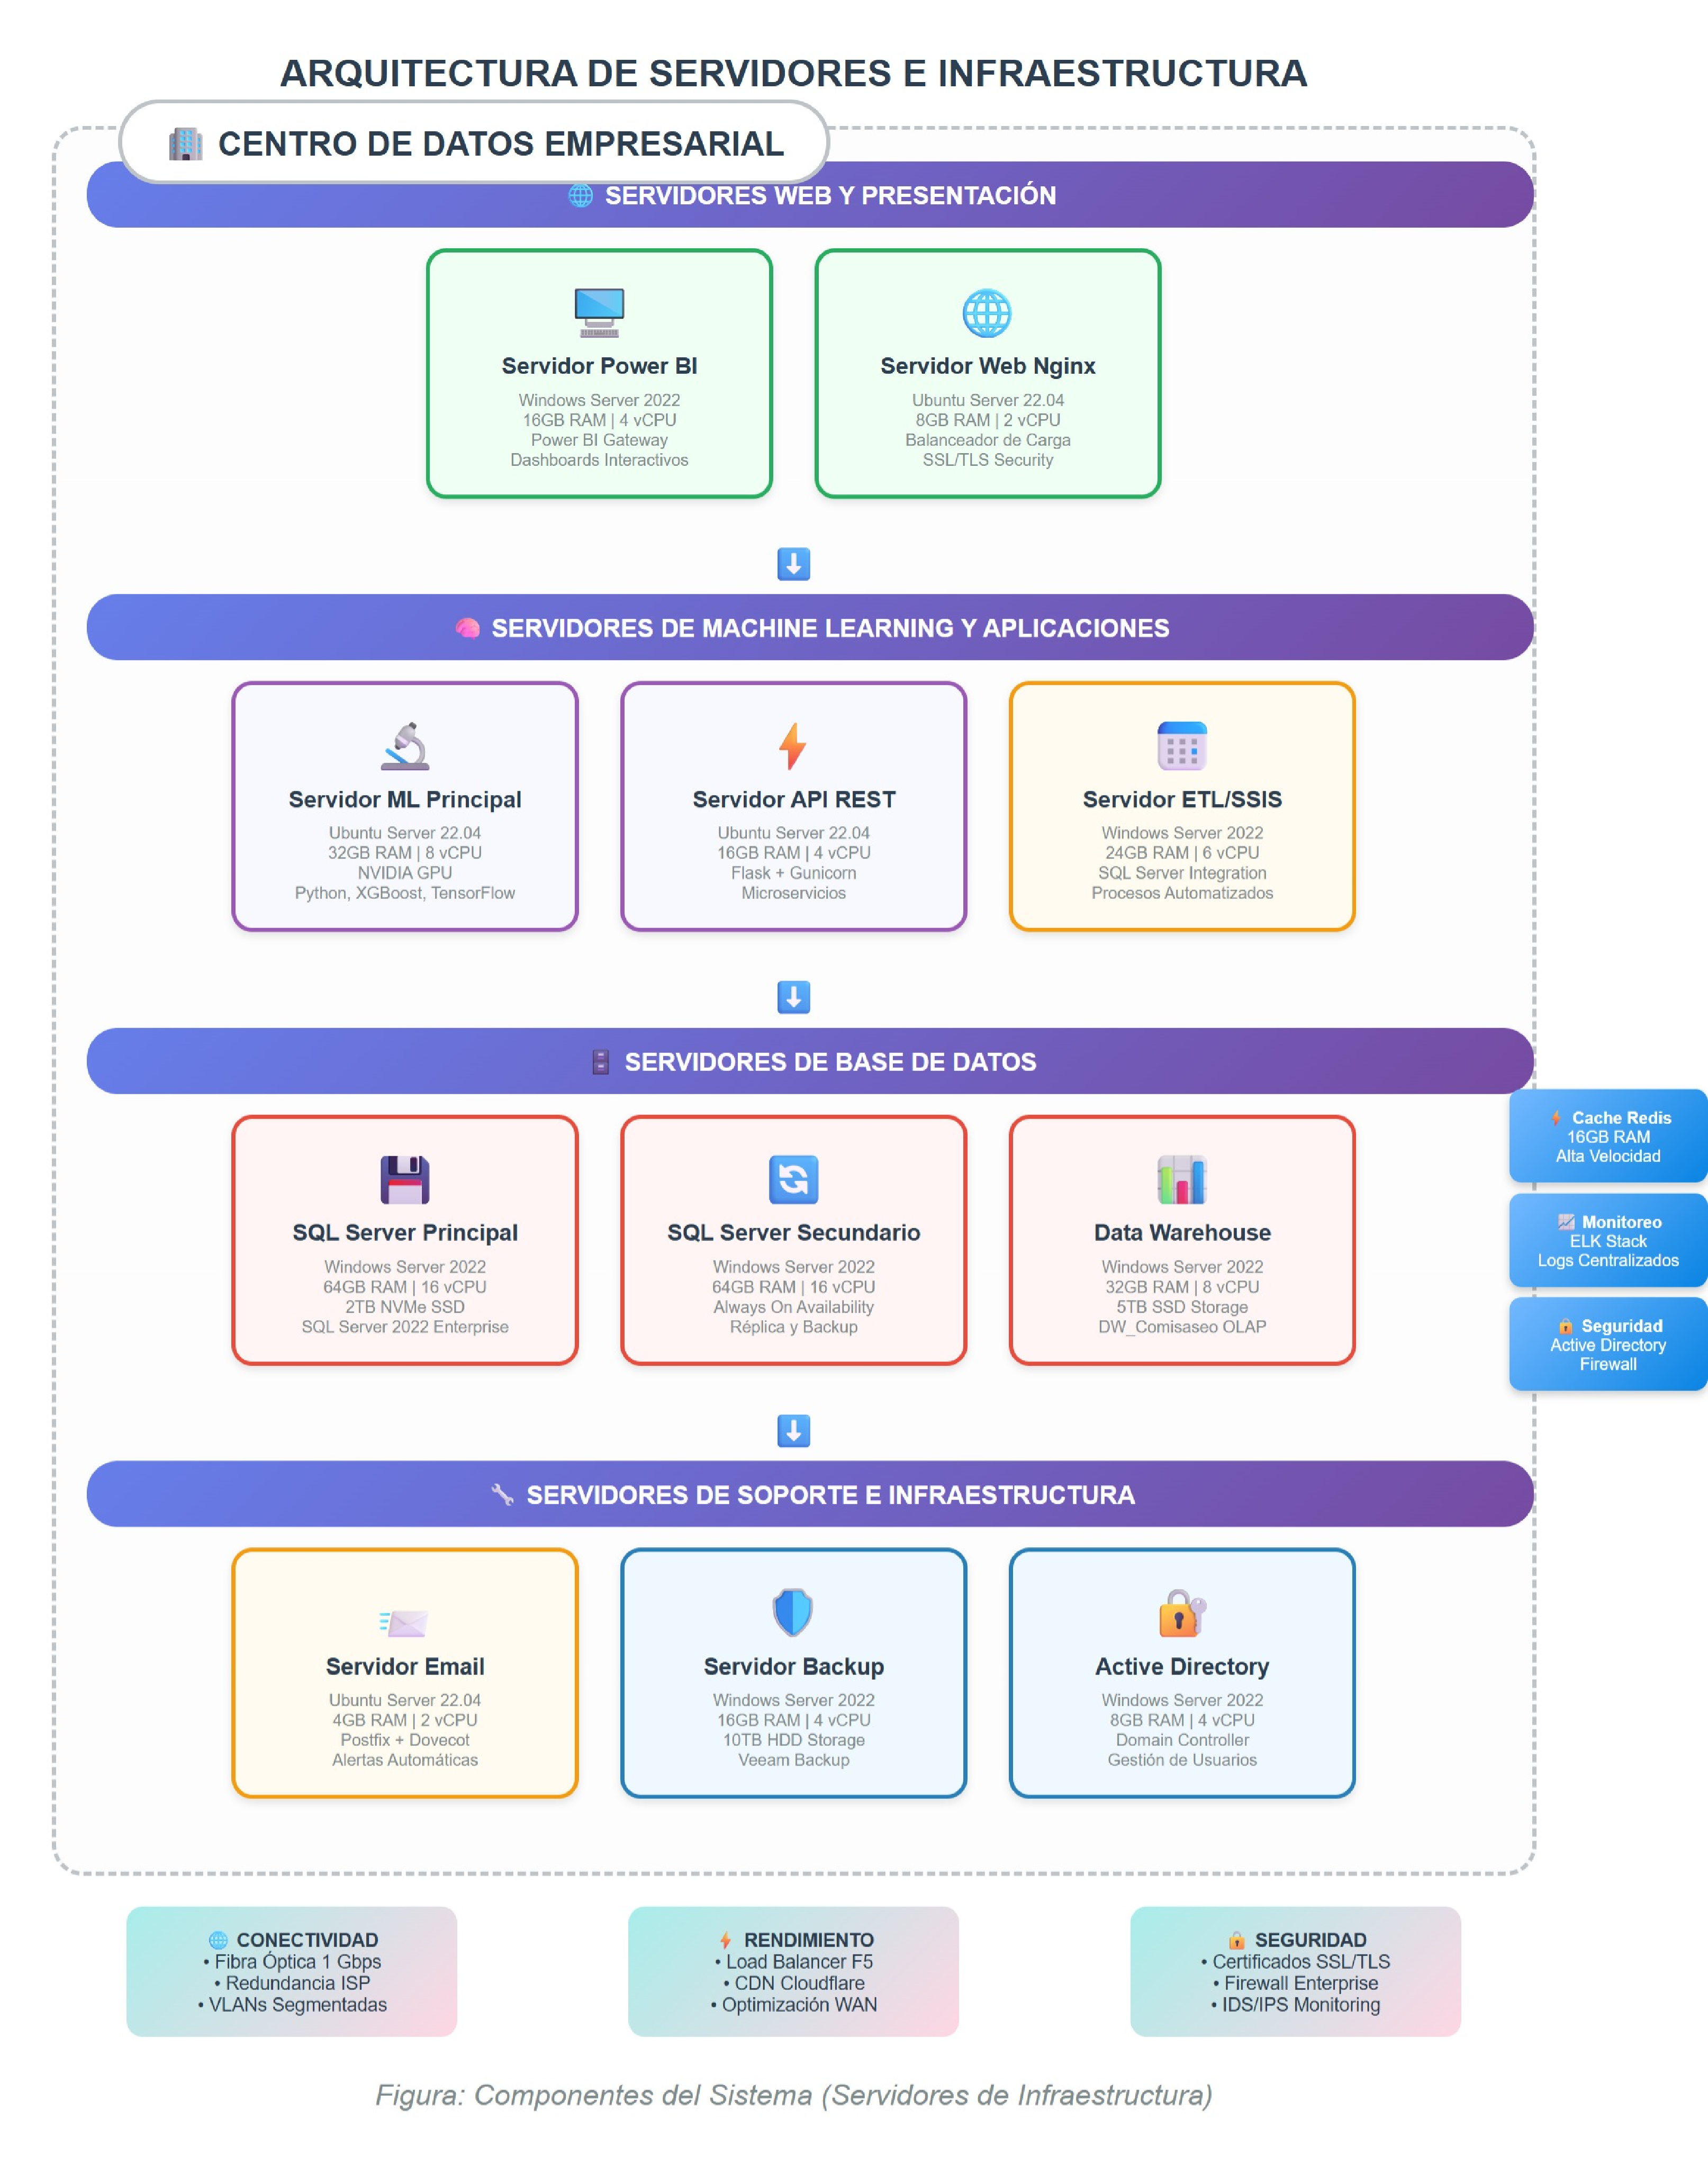
\includegraphics[width=1\textwidth,height=1\textheight,keepaspectratio]{Arquitectura de Servidores.pdf}
    \caption{Infraestructura de Tecnología}
    \label{fig:enter-label}
    \end{figure}
    \vfill
    \newpage

\subsection{Arquitectura de tecnología}

La arquitectura tecnológica implementada para el proyecto de predicción de morosidad se basa en un enfoque modular y escalable que permite la integración efectiva de técnicas de machine learning con sistemas empresariales existentes.


        
\subsubsection{Arquitectura de componentes}

El sistema se estructura en cinco capas principales que garantizan la separación de responsabilidades y facilitan el mantenimiento:

\begin{table}[ht]
\centering
\begin{tabular}{|p{3cm}|p{4cm}|p{7cm}|}
\hline
\textbf{Capa} & \textbf{Tecnología} & \textbf{Descripción} \\
\hline
Datos & SQL Server 2022, SSIS & Almacenamiento transaccional y histórico, procesos ETL automatizados \\
\hline
Integración & Python 3.9, pyodbc & Conectores de base de datos, APIs de integración \\
\hline
Procesamiento & Scikit-learn, XGBoost, Pandas & Motor de machine learning, preprocesamiento de datos \\
\hline
Servicios & Flask/FastAPI, REST & APIs para predicciones, servicios web \\
\hline
Presentación & Power BI, HTML5, JavaScript & Dashboards interactivos, reportes \\
\hline
\end{tabular}
\caption{Arquitectura de componentes del sistema}
\end{table}
 
\vfill
    \begin{figure}
    \centering    \includegraphics[width=1\textwidth,height=1\textheight,keepaspectratio]{Arquitectura de Tecnologías.pdf}
    \caption{Arquitectura de Tecnología}
    \label{fig:enter-label}
    \end{figure}
    \vfill
    \newpage 
   

\subsubsection{Infraestructura de despliegue}

\begin{itemize}
    \item \textbf{Servidor de Base de Datos:} 
    \begin{itemize}
        \item Windows Server 2019
        \item SQL Server 2022 Developer Edition
        \item 16 GB RAM, 4 vCPU
        \item Almacenamiento SSD 500 GB
    \end{itemize}
    
    \item \textbf{Servidor de Aplicaciones:}
    \begin{itemize}
        \item Ubuntu Server 20.04 LTS
        \item Python 3.9 con entorno virtual
        \item 8 GB RAM, 2 vCPU
        \item Nginx como proxy reverso
    \end{itemize}
    
    \item \textbf{Servidor de Visualización:}
    \begin{itemize}
        \item Power BI Service (Cloud)
        \item Gateway on-premises para conectividad
        \item Actualizaciones programadas cada 4 horas
    \end{itemize}
\end{itemize}

\subsubsection{Flujo de datos}

El flujo de datos sigue un patrón ETL (Extract, Transform, Load) optimizado:

\begin{enumerate}
    \item \textbf{Extracción:} Los datos se extraen de las vistas SQL Server mediante consultas programadas
    \item \textbf{Transformación:} Python procesa y normaliza los datos aplicando las transformaciones del modelo
    \item \textbf{Carga:} Los resultados se almacenan en tablas específicas para el modelo ML
    \item \textbf{Predicción:} El modelo XGBoost genera predicciones que se almacenan con timestamp
    \item \textbf{Visualización:} Power BI consume los datos procesados para generar dashboards
\end{enumerate}

\subsubsection{Seguridad y acceso}

\begin{itemize}
    \item \textbf{Autenticación:} Integrada con Active Directory de la empresa
    \item \textbf{Encriptación:} TLS 1.3 para todas las comunicaciones
    \item \textbf{Control de acceso:} Roles diferenciados por departamento
    \item \textbf{Auditoría:} Log de todas las predicciones y accesos al sistema
\end{itemize}
\section{Consideraciones Éticas y de Seguridad}
\subsection{Manejo de datos sensibles}
El proyecto implementa las siguientes medidas para el manejo ético de datos:

\begin{itemize}
    \item Anonimización de identificadores personales directos
    \item Agregación de datos para análisis que no requieren granularidad individual
    \item Almacenamiento encriptado de información sensible
    \item Política de acceso restrictivo basada en necesidad de conocimiento
    \item Documentación de flujos de datos y responsables de procesamiento
\end{itemize}

\section{Consideraciones Éticas y de Seguridad}

\subsection{Manejo de datos sensibles y confidencialidad}
El presente proyecto de investigación utiliza datos reales de transacciones comerciales y comportamiento de pago de clientes de una empresa mayorista ecuatoriana. Dada la naturaleza confidencial de esta información, se implementaron protocolos estrictos de manejo de datos que garantizan tanto la integridad de la investigación como la protección de la privacidad de los actores involucrados.

Se estableció un acuerdo formal de confidencialidad con la empresa participante, donde se especificaron los siguientes compromisos:

\begin{itemize}
    \item \textbf{Utilización exclusivamente académica:} Los datos se utilizan únicamente para fines académicos relacionados con el presente trabajo de titulación, sin ningún propósito comercial o transferencia a terceros.
    
    \item \textbf{Anonimización de información identificable:} Se aplicaron técnicas de anonimización mediante la asignación de códigos numéricos en lugar de nombres reales de clientes. La razón social de la empresa no se menciona en ninguna publicación derivada del trabajo.
    
    \item \textbf{Protección de información sensible:} Todas las cadenas de conexión, credenciales de acceso, y nombres de servidores presentados en el código y anexos utilizan valores genéricos ilustrativos (por ejemplo, \texttt{servidor-sqlserver}, \texttt{usuario\_analisis}) que no corresponden a las credenciales reales utilizadas durante el proyecto. Esta práctica es estándar en publicaciones académicas que involucran datos empresariales confidenciales \cite{barocas2016big}.
    
    \item \textbf{Compromiso de destrucción:} Al concluir el proyecto de investigación, los datos serán destruidos de manera segura o devueltos a la empresa, según lo establecido en el acuerdo de confidencialidad.
\end{itemize}

\subsubsection{Protocolos de seguridad implementados}
Los datos fueron almacenados en un ambiente seguro con las siguientes medidas de protección:

\begin{itemize}
    \item Acceso restringido mediante autenticación de múltiples factores
    \item Encriptación de datos en reposo utilizando algoritmos AES-256
    \item Procesamiento en entorno aislado sin conexión a redes públicas durante las fases de análisis
    \item Registro de auditoría de todos los accesos a los datos sensibles
    \item Backups encriptados con almacenamiento separado de las claves de acceso
\end{itemize}

\subsubsection{Contexto de la fuente de datos}
Aunque el documento de tesis describe conceptualmente la extracción de datos de múltiples fuentes (sistemas ERP para transacciones, sistemas CRM para información de clientes), la implementación técnica trabajó con vistas consolidadas ya preparadas por el equipo de tecnología de la empresa. Esta práctica es común en proyectos de investigación aplicada donde la empresa proporciona acceso a datos estructurados para facilitar el análisis, en lugar de otorgar acceso directo a sistemas transaccionales de producción.

Las vistas consolidadas fueron creadas por el equipo de TI de la empresa específicamente para este proyecto, asegurando que contengan únicamente la información necesaria para el análisis sin exponer datos operacionales sensibles adicionales. Este enfoque no invalida la investigación, sino que representa una buena práctica de gobernanza de datos y debe estar explícitamente documentado.

\subsection{Sesgos potenciales y estrategias de mitigación}
Los modelos de machine learning pueden inadvertidamente perpetuar o amplificar sesgos presentes en los datos históricos, resultando en decisiones discriminatorias o inequitativas \cite{barocas2016big}. En el contexto de predicción de morosidad, es crucial identificar y mitigar sesgos que podrían afectar injustamente a ciertos grupos de clientes.

Se implementaron las siguientes estrategias de mitigación de sesgos:

\begin{itemize}
    \item \textbf{Análisis de equidad geográfica:} Evaluación de la distribución de predicciones por región para verificar que el modelo no discrimine sistemáticamente contra clientes de zonas específicas debido a factores socioeconómicos externos a su control individual.
    
    \item \textbf{Evaluación desagregada de rendimiento:} Cálculo de tasas de falsos positivos y falsos negativos desagregadas por segmento de cliente para identificar disparidades en el rendimiento del modelo que pudieran afectar injustamente a ciertos grupos.
    
    \item \textbf{Validación de variables predictoras:} Verificación de que las variables utilizadas en el modelo están relacionadas con comportamiento de pago demostrable y no con características protegidas o proxies de las mismas.
    
    \item \textbf{Ausencia de variables demográficas sensibles:} Durante la fase de comprensión de los datos, se verificó que variables demográficas sensibles como género, etnia o religión no estuvieran presentes en el dataset, eliminando el riesgo de discriminación directa basada en estas características.
\end{itemize}

    Las variables geográficas incluidas (región, ciudad) están justificadas por su relación demostrable con factores económicos que afectan legítimamente el comportamiento de pago, como ciclos económicos regionales y patrones de estacionalidad del comercio local, no por características intrínsecas de las poblaciones de esas regiones.
    
    Se identifican además los siguientes sesgos potenciales y sus correspondientes estrategias de mitigación:
    
\begin{table}[h]
\centering
\begin{tabular}{|p{4cm}|p{5cm}|p{5cm}|}
\hline
\textbf{Tipo de sesgo} & \textbf{Manifestación potencial} & \textbf{Estrategia de mitigación} \\
\hline
Sesgo geográfico & Predicciones más precisas para regiones con mayor representación en los datos & Estratificación y ponderación de muestras por región \\
\hline
Sesgo temporal & Menor precisión en periodos atípicos o estacionales & Inclusión explícita de variables temporales y estacionales \\
\hline
Sesgo de selección & Sobrerrepresentación de clientes con mayor historial & Técnicas de balanceo para nuevos clientes vs. antiguos \\
\hline
Sesgo de confirmación & Tendencia a mantener patrones de evaluación preexistentes & Validación cruzada y evaluación por múltiples criterios \\
\hline
\end{tabular}
\caption{Sesgos potenciales y estrategias de mitigación}

\end{table}



\FloatBarrier
\subsection{Cumplimiento normativo}
En Ecuador, el manejo de información crediticia y datos personales está regulado por diversas normativas que buscan proteger los derechos de los individuos mientras permiten el desarrollo de la actividad comercial y financiera legítima. El desarrollo e implementación del modelo predictivo considera el cumplimiento de:

\begin{itemize}
    \item \textbf{Ley Orgánica de Protección de Datos Personales:} Aunque pendiente de promulgación completa al momento de este estudio, se consideraron los principios establecidos en el proyecto de ley, incluyendo finalidad legítima, proporcionalidad y transparencia en el tratamiento de datos.
    
    \item \textbf{Normativas de la Superintendencia de Compañías:} Cumplimiento de requisitos sobre reportes de cartera y manejo de información financiera comercial.
    
    \item \textbf{Políticas internas de confidencialidad:} Adherencia estricta a las políticas internas de la empresa sobre manejo de información y datos de clientes.
    
    \item \textbf{Estándares internacionales:} Consideración de mejores prácticas basadas en estándares internacionales de seguridad de información (ISO 27001) y principios de ética en inteligencia artificial.
\end{itemize}

\subsubsection{Principios normativos aplicados}
El presente proyecto se desarrolló considerando los siguientes principios fundamentales del tratamiento de datos:

\begin{itemize}
    \item \textbf{Finalidad legítima:} Uso de datos para fines de investigación académica orientada a mejorar prácticas de gestión comercial, sin propósitos discriminatorios ni perjudiciales para los titulares de los datos.
    
    \item \textbf{Proporcionalidad:} Recolección de datos limitada estrictamente a variables relevantes para el objetivo de investigación, sin captura de información innecesaria o excesiva.
    
    \item \textbf{Transparencia:} Documentación clara y completa de las metodologías, fuentes de datos utilizadas, y procedimientos aplicados, permitiendo auditoría y verificación externa.
    
    \item \textbf{Titularidad y legitimación:} Los datos fueron proporcionados por la empresa en su calidad de titular de la información de sus relaciones comerciales. El análisis se realizó con fines internos de mejora de procesos sin transferencia a terceros ni uso comercial externo, enmarcándose dentro de las excepciones previstas en la normativa vigente para procesamiento interno y análisis estadístico.
\end{itemize}